
% Beamer Presentation

\documentclass{beamer}
\mode<presentation> {
% Theme
\usetheme{metropolis}
%\setbeamertemplate{footline} % To remove the footer line in all slides uncomment this line
%\setbeamertemplate{footline}[page number] % To replace the footer line in all slides with a simple slide count uncomment this line
%\setbeamertemplate{navigation symbols}{} % To remove the navigation symbols from the bottom of all slides uncomment this line
}

%Packages
\usepackage{graphicx} % Allows including images
\usepackage{booktabs} % Allows the use of \toprule, \midrule and \bottomrule in tables
%\usepackage{cite}
\usepackage[numbers]{natbib} % For bibliography
\usepackage{multirow}
\usepackage{hyperref}
%\usetheme{Warsaw}
\usepackage[absolute,overlay]{textpos}
\usepackage{xcolor}


% Colors
%\definecolor{Red}{rgb}{0.7,0,0}
%\definecolor{Blue}{rgb}{0,0,0.8}

% Prepare title and TOC
\title[Short title]{Introduction to R} 
\author{Marco Chiapello} 
\institute[Center for Proteomics] 
{
Center for Proteomics\\
University of Cambridge \\ 
\medskip
\textit{mc983@cam.ac.uk} 
}
\date{\today} 

%\AtBeginSection[]
%{
%\begin{frame}<beamer>
%\frametitle{Overview}
%\tableofcontents[currentsection]
%\end{frame}
%}


%-------------------------------------------
% MAIN DOCUMENT
%-------------------------------------------
\usepackage{Sweave}
\begin{document}
\Sconcordance{concordance:Rbasic_Day1.tex:Rbasic_Day1.Rnw:%
1 54 1 1 0 184 1 1 2 6 0 1 1 5 0 1 1 5 0 1 1 6 0 1 2 9 1 1 2 7 0 1 2 11 %
1 1 2 1 0 1 1 6 0 1 2 2 1 1 2 1 0 1 1 6 0 1 2 7 1 1 2 7 0 1 2 2 1 1 2 6 %
0 2 1 6 0 1 2 8 1 1 2 6 0 1 1 5 0 1 1 6 0 1 2 8 1 1 2 1 0 1 1 6 0 1 2 %
15 1 1 2 7 0 1 2 8 1 1 2 7 0 1 2 10 1 1 2 7 0 1 2 20 1 1 2 7 0 1 2 9 1 %
1 2 7 0 1 2 9 1 1 2 1 0 1 1 6 0 1 2 9 1 1 2 7 0 1 2 14 1 1 2 7 0 1 2 7 %
1 1 2 7 0 1 2 3 1 1 2 7 0 1 2 10 1 1 3 8 0 1 2 11 1 1 3 8 0 1 2 9 1 1 3 %
8 0 1 2 18 1 1 2 7 0 1 2 9 1 1 2 6 0 1 1 6 0 1 2 9 1 1 2 6 0 1 1 6 0 1 %
2 9 1 1 2 1 0 1 1 5 0 1 1 5 0 1 2 7 0 1 2 7 1 1 2 1 0 2 1 6 0 1 2 8 1 1 %
2 1 0 1 1 6 0 1 2 3 1 1 2 6 0 1 1 6 0 1 2 9 1 1 2 1 0 1 1 6 0 1 2 5 1 1 %
2 1 0 1 1 5 0 2 1 7 0 1 2 57 1 1 2 1 0 1 1 1 2 1 0 2 1 3 0 1 2 5 1 1 2 %
1 0 1 1 7 0 1 2 12 1 1 2 1 0 1 1 7 0 1 2 5 1 1 2 7 0 1 1 7 0 1 2 12 1 1 %
2 1 0 1 1 6 0 1 2 105 1 1 13 1 2 17 0 1 2 10 1 1 2 1 0 1 1 3 0 1 2 6 1 %
1 3 2 0 1 2 4 0 1 2 6 1 1 2 4 0 1 2 12 1 1 2 7 0 1 2 7 1 1 2 6 0 1 1 5 %
0 1 1 5 0 1 1 6 0 1 2 18 1 1 2 7 0 1 1 7 0 1 2 18 1 1 3 2 0 1 1 16 0 1 %
2 5 1 1 2 7 0 1 2 14 1 1 3 2 0 1 1 7 0 1 2 5 1 1 4 3 0 1 1 7 0 1 2 13 1 %
1 2 1 0 1 1 11 0 2 2 1 0 1 1 8 0 1 2 18 1 1 2 1 0 4 1 9 0 1 2 2 1 1 2 7 %
0 1 2 19 1 1 2 8 0 1 2 2 1 1 2 8 0 2 2 9 0 1 2 16 1 1 2 6 0 1 1 6 0 1 2 %
18 1 1 2 1 0 1 1 5 0 1 1 5 0 2 1 5 0 1 1 5 0 1 1 5 0 1 1 6 0 1 2 68 1 1 %
2 1 0 6 1 16 0 1 2 18 1 1 2 7 0 1 2 8 1 1 2 1 0 1 1 5 0 2 1 10 0 1 1 6 %
0 1 2 1 1 1 2 6 0 1 1 5 0 1 1 6 0 1 2 16 1 1 2 7 0 1 2 8 1 1 2 10 0 1 2 %
8 1 1 2 7 0 1 2 16 1 1 2 1 0 1 1 7 0 1 2 8 1 1 2 1 0 1 1 6 0 1 1 5 0 1 %
1 7 0 1 2 126 1 1 2 1 0 1 1 5 0 2 1 5 0 1 1 3 0 1 2 13 1 1 2 1 0 1 1 9 %
0 1 1 505 0 1 2 39 1 1 2 1 0 2 1 505 0 1 2 23 1 1 2 1 0 1 1 6 0 1 2 113 %
1 1 2 4 0 1 2 212 1}

\newlength{\fancyvrbtopsep}
\newlength{\fancyvrbpartopsep}
\makeatletter
\FV@AddToHook{\FV@ListParameterHook}{\topsep=\fancyvrbtopsep\partopsep=\fancyvrbpartopsep}
\makeatother
\setlength{\fancyvrbtopsep}{-3pt}
\setlength{\fancyvrbpartopsep}{-3pt}

%-------------------------------------------
% TITLE PAGE
%-------------------------------------------
\begin{frame}
	\titlepage 
\end{frame}

%-------------------------------------------
% TABLE OF CONTENTS
%-------------------------------------------
\begin{frame}{Overview}
	\small
	\tableofcontents
\end{frame}

%----------------------------------------------------------------------------------------
%	PRESENTATION SLIDES
%----------------------------------------------------------------------------------------

%-------------------
% INTRODUCTION
%-------------------
\section{Introduction}

%%%%%%% 
\begin{frame}
	\frametitle{What R is?}
	\Large The \texttt{R} Project for Statistical Computing
	\begin{itemize}
		\small
		\item \texttt{R} is a free software environment for statistical computing and graphics
		\item Open source and cross platform (UNIX platforms, Windows and MacOS)
		\item Extensive graphics capabilities
		\item Diverse range of add-on packages
		\item Active community of developers
		\item Thorough documentation
	\end{itemize}
\end{frame}

%%%%%%% 
\begin{frame}
	\frametitle{What R is?}
        \Large The \texttt{R} Project for Statistical Computing\\
	\small You can find \texttt{R} here:
	\url{https://www.r-project.org}\\
	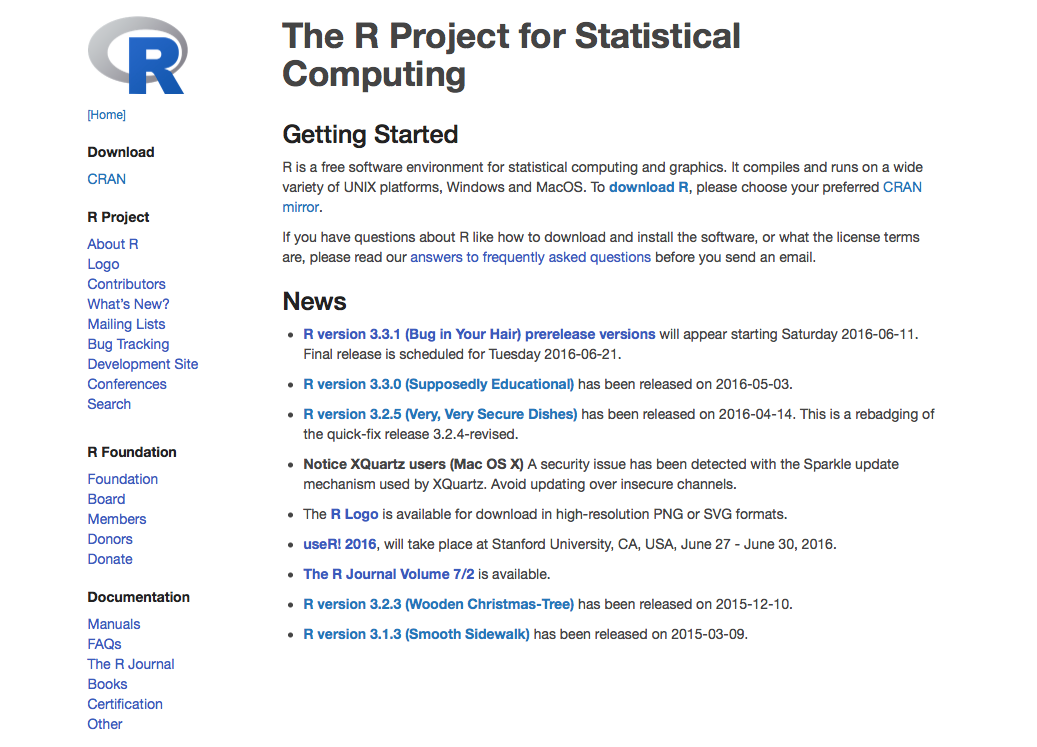
\includegraphics[scale=0.25]{figures/R-project.png}
\end{frame}

%%%%%%% 
\begin{frame}
	\frametitle{What R is?}
        \Large The \texttt{R} Project for Statistical Computing\\
	\begin{itemize}
		\small
		\item R version 3.3.1 (released 2016-06-21)
		\item Currently, the CRAN {\tiny(Comprehensive R Archive Network)} package repository features 8609 available packages
			\begin{itemize}
				\item \tiny \url{https://cran.r-project.org/web/packages/available_packages_by_name.html}
			\end{itemize}
		\item Currently, the Bioconductor repository features 1211 available packages
			\begin{itemize}
				\item \tiny \url{http://www.bioconductor.org}
			\end{itemize}
		\item Executed using command line, or a graphical user interface (GUI)
		\item On this course, we use the RStudio GUI
			\begin{itemize}
				\item \tiny \url{www.rstudio.com}
			\end{itemize}
	\end{itemize}
\end{frame}

%%%%%%% 
\begin{frame}[fragile]
	\frametitle{Getting started}
        \begin{itemize}
          \item \texttt{R} is a program which, once installed on your system, can be launched and is immediately ready to take input directly from the user
          \item There are two ways to launch R:
            \begin{enumerate}
              \small
              \item From the command line (particularly useful if you're quite familiar with Linux)
              \item As an application called RStudio (very good for beginners)
            \end{enumerate}
        \end{itemize}
\end{frame}

%%%%%%% 
\begin{frame}
	\frametitle{Launch R}
  \texttt{R} can be launched in 2 ways:
  \begin{enumerate}
    \item From command line
      \begin{itemize}
        \item To start \texttt{R} you need to enter the console (also called terminal or shell)
        \item To start \texttt{R}, at the prompt simply type: \Large \texttt{R}
      \end{itemize}
    \item Using RStudio
      \begin{itemize}
          \item To launch RStudio, find the RStudio icon and double-click
        \end{itemize}
  \end{enumerate}
\end{frame}

%%%%%%% 
\begin{frame}
	\frametitle{RStudio}
	Since we will use RStudio in this course, let's have a look of the program\\
	\centering 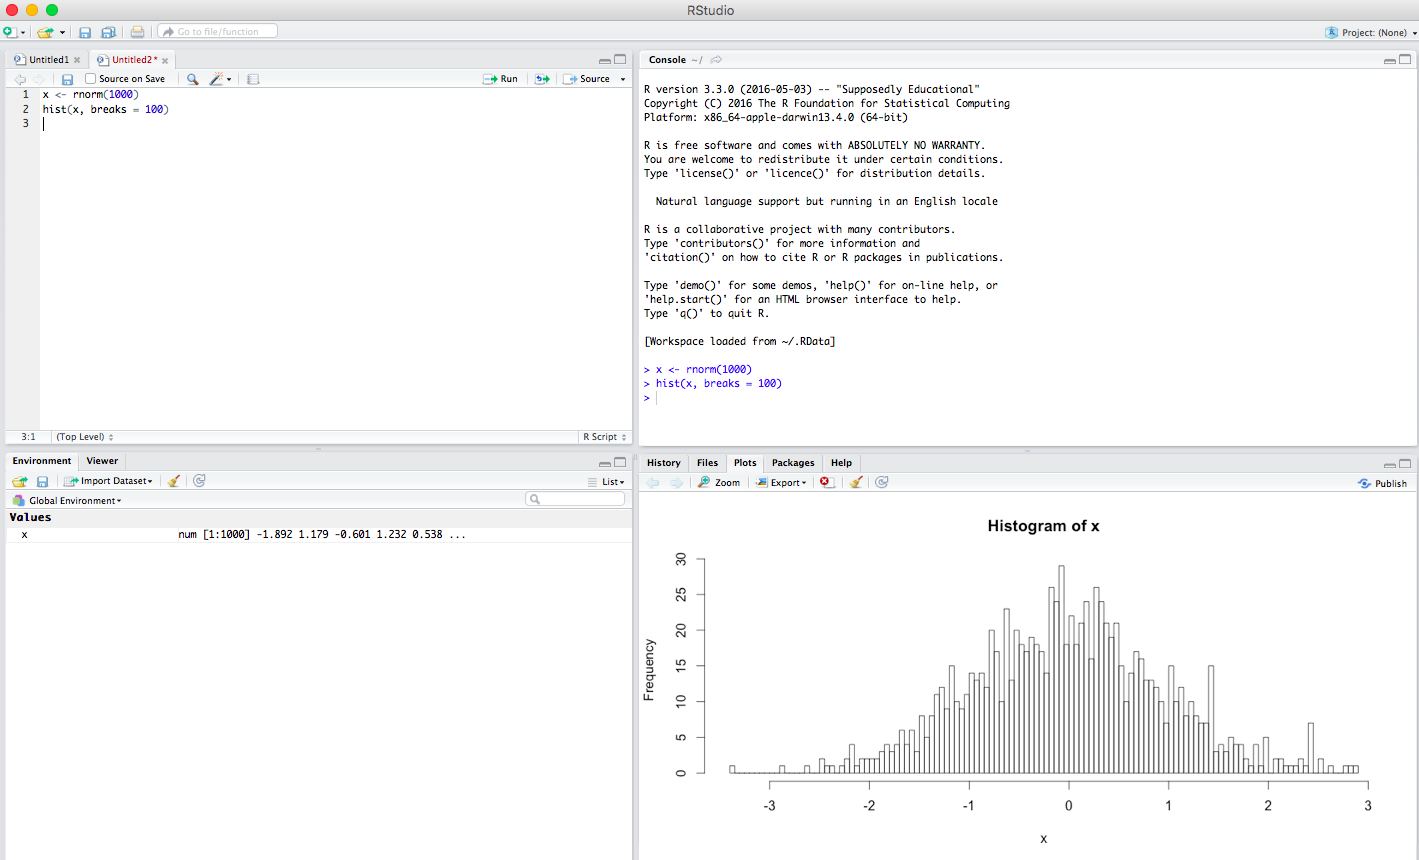
\includegraphics[scale=1.4]{figures/Rstudio_overview.png}
\end{frame}

%%%%%%% 
\begin{frame}
	\frametitle{RStudio}
	\textbf{R console}\\
	\vspace{20pt}
	\centering 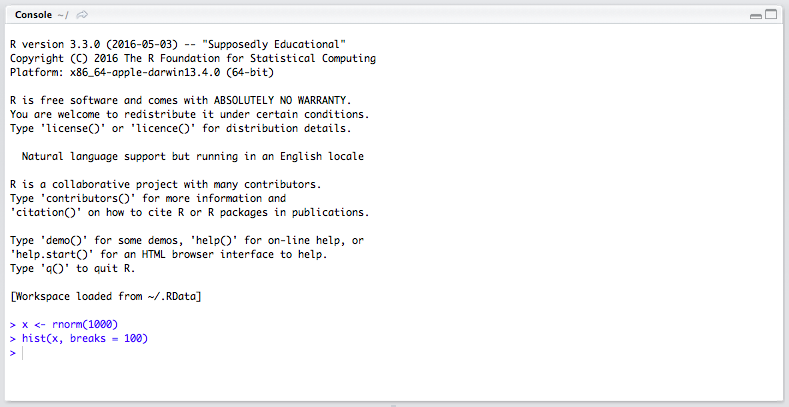
\includegraphics[width=11cm]{figures/RStudio_console.png}\\
	\small It is the place where you can interactively run R commands
\end{frame}

%%%%%%% 
\begin{frame}
	\frametitle{RStudio}
	\textbf{Source editor for R scripts}\\
	\vspace{20pt}
	\centering 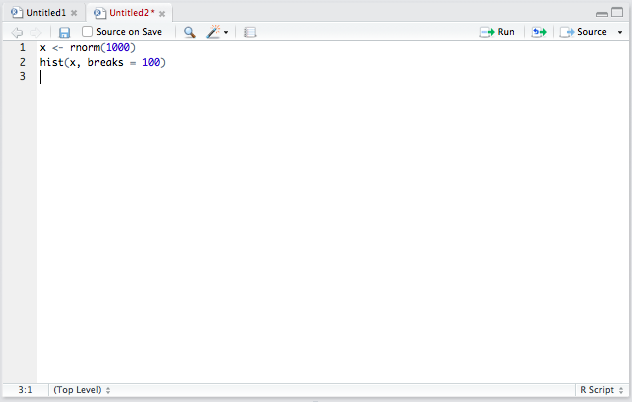
\includegraphics[width=10cm]{figures/RStudio_script.png}\\
	\small It is the place where you can write your scripts
\end{frame}

%%%%%%% 
\begin{frame}
	\frametitle{RStudio}
	\textbf{Workspace}\\
	\vspace{16pt}
	\centering 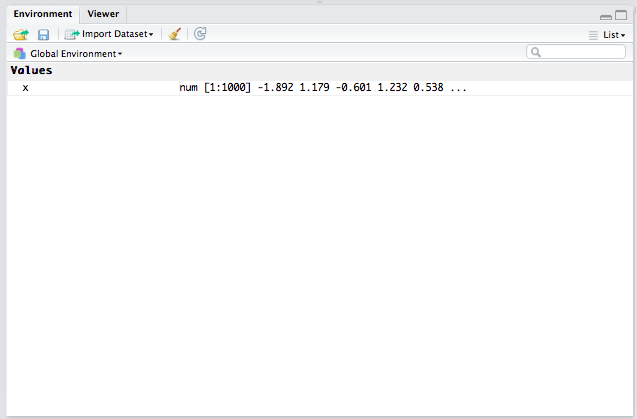
\includegraphics[width=10cm]{figures/RStudio_environment.png}\\
	\small It is the place where you can view object in the global environment
\end{frame}

%%%%%%% 
\begin{frame}
	\frametitle{RStudio}
	\textbf{Plot pannel}\\
	\vspace{20pt}
	\centering 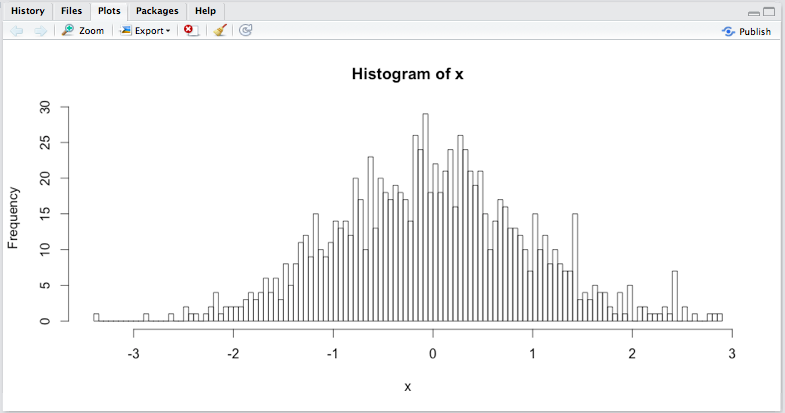
\includegraphics[width=10cm]{figures/RStudio_plot.png}\\
	\small It is the place where you can view your plots
\end{frame}

%%%%%%% 
\begin{frame}
	\frametitle{RStudio}
	\textbf{R help}\\
	\vspace{20pt}
	\centering 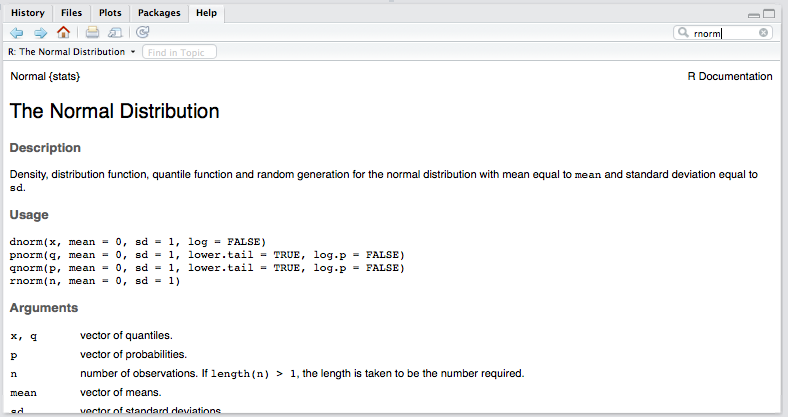
\includegraphics[width=10cm]{figures/RStudio_help.png}\\
	\small It is the place where you can find help
\end{frame}

%%%%%%% 
\begin{frame}
	\frametitle{RStudio}
	The GUI is divided into 4 main sub-windows\\
	These sub-windows are customizable\\
	\vspace{10pt}
	\centering 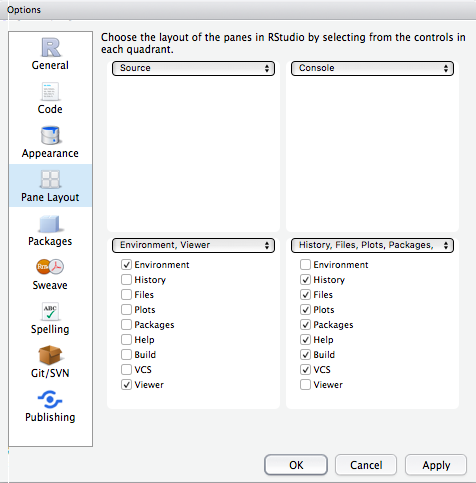
\includegraphics[width=7cm]{figures/RStudio_option.png}
\end{frame}

%%%%%%%%%%%%%%%%%%%%%%%%%%%%%%%%%%%%%%%%%%%%%%%%%%%%%%%%%%%%%%%%%%%%%%
%%%%%%%%%%%%%%%%%%%%%%%%%%%%%%%%%%%%%%%%%%%%%%%%%%%%%%%%%%%%%%%%%%%%%%
\section{Basic concepts in R}

%%%%%%% 
\begin{frame}[fragile]{prova}
	\frametitle{Numbers}
	The command line can be used as a calculator
\rule{\textwidth}{0.4pt}
\begin{Schunk}
\begin{Sinput}
> 5 + 7 
\end{Sinput}
\begin{Soutput}
[1] 12
\end{Soutput}
\begin{Sinput}
> 5 - 7
\end{Sinput}
\begin{Soutput}
[1] -2
\end{Soutput}
\begin{Sinput}
> 5 * 7
\end{Sinput}
\begin{Soutput}
[1] 35
\end{Soutput}
\begin{Sinput}
> 5 / 7
\end{Sinput}
\begin{Soutput}
[1] 0.7142857
\end{Soutput}
\end{Schunk}
\rule{\textwidth}{0.4pt}
\vspace{5pt}
\small Note: The number in the square brackets is an indicator of the position in the output
\end{frame}

%%%%%%% 
\begin{frame}[fragile]{prova}
	\frametitle{Numbers}
	You can solve simple or complex calculations 
	\rule{\textwidth}{0.4pt}
\begin{Schunk}
\begin{Sinput}
> (((20/5)^2)-((5+1/3+4/5-10)*(2-34))-20)
\end{Sinput}
\begin{Soutput}
[1] -127.7333
\end{Soutput}
\end{Schunk}
\rule{\textwidth}{0.4pt}
\vspace{20pt}
\Large But, of course, \texttt{R} is not a calculator
\end{frame}

%%%%%%% 
\begin{frame}[fragile]
	\frametitle{Variables}
	A \textbf{variable} is a letter or word which takes (or contains) a value. We use the assignment 'operator', <-\\
	\vspace{10pt}
	- We can assign a number to a variable
	\rule{\textwidth}{0.4pt}
\begin{Schunk}
\begin{Sinput}
> x <- 5
> x
\end{Sinput}
\begin{Soutput}
[1] 5
\end{Soutput}
\end{Schunk}
 \rule{\textwidth}{0.4pt}
 - We can assign the result of an operation to a variable
 \rule{\textwidth}{0.4pt}
\begin{Schunk}
\begin{Sinput}
> y <- 5 + 7
> y
\end{Sinput}
\begin{Soutput}
[1] 12
\end{Soutput}
\end{Schunk}
\rule{\textwidth}{0.4pt}
\end{frame}

%%%%%%% 
\begin{frame}[fragile]
	\frametitle{Variables}
	- We can assign use the variables to perform calculation
	\rule{\textwidth}{0.4pt}
\begin{Schunk}
\begin{Sinput}
> x + y
\end{Sinput}
\begin{Soutput}
[1] 17
\end{Soutput}
\end{Schunk}
 \rule{\textwidth}{0.4pt}
 - We can assign the change the content of the variable
 \rule{\textwidth}{0.4pt}
\begin{Schunk}
\begin{Sinput}
> x
\end{Sinput}
\begin{Soutput}
[1] 5
\end{Soutput}
\begin{Sinput}
> x <- x - y
> x
\end{Sinput}
\begin{Soutput}
[1] -7
\end{Soutput}
\end{Schunk}
\rule{\textwidth}{0.4pt}
\end{frame}

%%%%%%% 
\begin{frame}[fragile]
	\frametitle{Function}
	\textbf{Functions} in \texttt{R} perform operations on arguments (the input(s) to the function). \\ Arguments are always contained in parentheses, i.e. curved brackets (), separated by commas.
	\vspace{10pt}
	
\begin{Schunk}
\begin{Sinput}
> sum(3, 4, 5, 6)
\end{Sinput}
\begin{Soutput}
[1] 18
\end{Soutput}
\begin{Sinput}
> max(3, 4, 5, 6)
\end{Sinput}
\begin{Soutput}
[1] 6
\end{Soutput}
\begin{Sinput}
> min(3, 4, 5, 6)
\end{Sinput}
\begin{Soutput}
[1] 3
\end{Soutput}
\end{Schunk}

\end{frame}

%%%%%%% 
\begin{frame}[fragile]
	\frametitle{Function extention}
	\texttt{R} contains a lot of pre-builtin functions, but through the so called \textit{packages} is possible extend the \texttt{R} functionalities enormously.
	\vspace{30pt}
	Alternatevely, you can write your own function
\begin{Schunk}
\begin{Sinput}
> summ <- function(a,b){ a + b }
> summ(1,2)
\end{Sinput}
\begin{Soutput}
[1] 3
\end{Soutput}
\end{Schunk}
\end{frame}



\subsection{Vector}
%%%%%%% 
\begin{frame}
	\centering \Huge Vector
\end{frame}

%%%%%%% 
\begin{frame}[fragile]
	\frametitle{Vector}
	The basic data structure in \texttt{R} is a \textbf{vector}, an ordered collection of values. \texttt{R} even treats single values as 1-element vectors.\\
	The simplest way to create a \textbf{vector} in \texttt{R} is by using the c() operator:
	\rule{\textwidth}{0.4pt}
\begin{Schunk}
\begin{Sinput}
> c(1,2,3,50)
\end{Sinput}
\begin{Soutput}
[1]  1  2  3 50
\end{Soutput}
\end{Schunk}
\rule{\textwidth}{0.4pt}
\vspace{20pt}
That gave us every integer between (and including) 1 and 10.
\end{frame}

%%%%%%% 
\begin{frame}[fragile]
	\frametitle{Vector}
	The simplest way to create a \textbf{sequence of numbers} is by using the `:` operator:
	\rule{\textwidth}{0.4pt}
\begin{Schunk}
\begin{Sinput}
> 1:10
\end{Sinput}
\begin{Soutput}
 [1]  1  2  3  4  5  6  7  8  9 10
\end{Soutput}
\end{Schunk}
\rule{\textwidth}{0.4pt}
\vspace{20pt}
That gave us every integer between (and including) 1 and 10.
\end{frame}

%%%%%%% 
\begin{frame}[fragile]
	\frametitle{Vector}
	What happens if we do 15:1? Give it a try to find out.
	\pause
	\rule{\textwidth}{0.4pt}
\begin{Schunk}
\begin{Sinput}
> 15:1
\end{Sinput}
\begin{Soutput}
 [1] 15 14 13 12 11 10  9  8  7  6  5  4  3  2  1
\end{Soutput}
\end{Schunk}
\rule{\textwidth}{0.4pt}\\
\vspace{20pt}
It counted backwards in increments of 1!
\end{frame}

%%%%%%% 
\begin{frame}[fragile]
	\frametitle{Vector}
  	Remember that if you have questions about a particular R function, you can access its documentation with a question mark followed by the function name:\\
\begin{equation}?function name here \end{equation}\\
  However, in the case of an operator like the colon used above, you must enclose the symbol in backticks like this:\\
  \begin{equation}?`: \end{equation}\\
\end{frame}

%%%%%%% 
\begin{frame}[fragile]
	\frametitle{Vector}
	Often, we'll desire more control over a sequence we're creating than what the `:` operator gives us. The seq() function serves this purpose.\\
	\centering Try it: \small Remember what we said about the function arguments\\
	\pause
	\rule{\textwidth}{0.4pt}
\begin{Schunk}
\begin{Sinput}
> seq(1,10)
\end{Sinput}
\begin{Soutput}
 [1]  1  2  3  4  5  6  7  8  9 10
\end{Soutput}
\end{Schunk}
	\rule{\textwidth}{0.4pt}
\end{frame}

%%%%%%% 
\begin{frame}[fragile]
	\frametitle{Vector}
	This gives us the same output as 1:20. However, let's say that instead we want a vector of numbers ranging from 0 to 4, incremented by 0.5. seq(0, 4,by=0.5) does just that.\\
	\centering Try it out.\\
	\pause
	\rule{\textwidth}{0.4pt}
\begin{Schunk}
\begin{Sinput}
> seq(0, 4, by = 0.5)
\end{Sinput}
\begin{Soutput}
[1] 0.0 0.5 1.0 1.5 2.0 2.5 3.0 3.5 4.0
\end{Soutput}
\end{Schunk}
\rule{\textwidth}{0.4pt}
\end{frame}

%%%%%%% 
\begin{frame}[fragile]
	\frametitle{Vector}
	Or maybe we don't care what the increment is and we just want a sequence of 10 numbers between 5 and 10. seq(5, 10, length=10) does the trick. Give it a shot now and store the result in a new variable called \textit{mySeq}.\\
	\centering Try it out.\\
	\pause
\rule{\textwidth}{0.4pt}
\begin{Schunk}
\begin{Sinput}
> mySeq <- seq(5, 10, length=10)
> round(mySeq,1)
\end{Sinput}
\begin{Soutput}
 [1]  5.0  5.6  6.1  6.7  7.2  7.8  8.3  8.9  9.4 10.0
\end{Soutput}
\end{Schunk}
  \rule{\textwidth}{0.4pt}
\end{frame}

%%%%%%% 
\begin{frame}[fragile]
\frametitle{Vector}
To confirm that mySeq has length 10, we can use the length() function.\\
\centering Try it now\\
\pause
\rule{\textwidth}{0.4pt}
\begin{Schunk}
\begin{Sinput}
> length(mySeq)
\end{Sinput}
\begin{Soutput}
[1] 10
\end{Soutput}
\end{Schunk}
  \rule{\textwidth}{0.4pt}
\end{frame}

%%%%%%% 
\begin{frame}[fragile]
	\frametitle{Vector}
	\begin{itemize}
  	\item Let's pretend we don't know the length of mySeq, but we want to generate a sequence of integers from 1 to N, where N represents the length of the mySeq vector.
  	\item We want a new vector (1, 2, 3, ...) that is the same length as mySeq.
  	\item There are several ways we could do this. 
  	\item One possibility is to combine the `:` operator and the length() function.
	\end{itemize}
	\centering Give that a try
	\pause
\rule{\textwidth}{0.4pt}
\begin{Schunk}
\begin{Sinput}
> 1:length(mySeq)
\end{Sinput}
\begin{Soutput}
 [1]  1  2  3  4  5  6  7  8  9 10
\end{Soutput}
\end{Schunk}
\rule{\textwidth}{0.4pt}
\end{frame}

%%%%%%% 
\begin{frame}[fragile]
	\frametitle{Vector}
	Another option is to use seq(along.with = mySeq). Give that a try.
\rule{\textwidth}{0.4pt}
\begin{Schunk}
\begin{Sinput}
> seq(along.with = mySeq)
\end{Sinput}
\begin{Soutput}
 [1]  1  2  3  4  5  6  7  8  9 10
\end{Soutput}
\end{Schunk}
\rule{\textwidth}{0.4pt}\\
\vspace{20pt}
R has a separate built-in function for this purpose
\rule{\textwidth}{0.4pt}
\begin{Schunk}
\begin{Sinput}
> seq_along(mySeq)
\end{Sinput}
\begin{Soutput}
 [1]  1  2  3  4  5  6  7  8  9 10
\end{Soutput}
\end{Schunk}
\rule{\textwidth}{0.4pt}
\end{frame}

%%%%%%% 
\begin{frame}[fragile]
	\frametitle{Vector}
	\begin{itemize}
	\item There are often \textbf{several approaches} to solving the same problem in \texttt{R}          \item Simple approaches that involve \textbf{less typing} are generally best
	\item It is also important for your code to be \textbf{readable}, so that you and others can figure out what's going on without too much hassle
	\end{itemize}
\rule{\textwidth}{0.4pt}
\begin{Schunk}
\begin{Sinput}
> # Create a sequence of 10 numbers
> seq_along(mySeq)
\end{Sinput}
\begin{Soutput}
 [1]  1  2  3  4  5  6  7  8  9 10
\end{Soutput}
\end{Schunk}
\rule{\textwidth}{0.4pt}
\small The comments in \texttt{R} begin with \textbf{hash}. You should have about 1/3 of your code commented. 
\end{frame}

%%%%%%% 
\begin{frame}[fragile]
	\frametitle{Vector}
	One more function related to creating sequences of numbers is rep(), which stands for 'replicate'.\\
	If we're interested in creating a vector that contains 1 and 0 five times, we can use rep(c(1,0), times = 5).\\
	\centering Try it out
	\pause
	\rule{\textwidth}{0.4pt}
\begin{Schunk}
\begin{Sinput}
> # Create a sequence of 1 and 0
> rep(c(1,0), times = 5)
\end{Sinput}
\begin{Soutput}
 [1] 1 0 1 0 1 0 1 0 1 0
\end{Soutput}
\end{Schunk}
\rule{\textwidth}{0.4pt}
\end{frame}

%%%%%%% 
\begin{frame}[fragile]
	\frametitle{Vector}
If we want our vector to contain 5 ones and then 5 zeros, we can do this with the `each` argument instead of `times` argument.\\
  \centering Try it out\\
  \pause
  \rule{\textwidth}{0.4pt}
\begin{Schunk}
\begin{Sinput}
> # Create a sequence of 1 and 0
> rep(c(1,0), each = 5)
\end{Sinput}
\begin{Soutput}
 [1] 1 1 1 1 1 0 0 0 0 0
\end{Soutput}
\end{Schunk}
\rule{\textwidth}{0.4pt}
\end{frame}

%%%%%%% 
\begin{frame}[fragile]
	\frametitle{Vector}
	\begin{itemize}
	\item We'll see, now, how to \textbf{extract} elements from a vector (subset)
	\item The square brackets \textbf{[]} indicate position within the vector
	  \begin{itemize}
	    \small
	    \item \texttt{R} even treats single values as 1-element vectors
	    \item The vector in \texttt{R} starts from position 1
	  \end{itemize}
	\item We can extract individual elements by using the \textbf{[]} notation
  \end{itemize}
  \centering Try mySeq[1:3]\\
  \pause
  \rule{\textwidth}{0.4pt}
\begin{Schunk}
\begin{Sinput}
> mySeq[1:3]
\end{Sinput}
\begin{Soutput}
[1] 5.000000 5.555556 6.111111
\end{Soutput}
\end{Schunk}
\rule{\textwidth}{0.4pt}
\end{frame}

%%%%%%% 
\begin{frame}[fragile]
	\frametitle{Vector}
	If we want to 3th, 5th and 10th elements of the vector mySeq.\\
	\centering Try it out
	\pause
	\rule{\textwidth}{0.4pt}
\begin{Schunk}
\begin{Sinput}
> round(mySeq,1)
\end{Sinput}
\begin{Soutput}
 [1]  5.0  5.6  6.1  6.7  7.2  7.8  8.3  8.9  9.4 10.0
\end{Soutput}
\begin{Sinput}
> round(mySeq[c(3,5,10)],1)
\end{Sinput}
\begin{Soutput}
[1]  6.1  7.2 10.0
\end{Soutput}
\end{Schunk}
  \rule{\textwidth}{0.4pt}
\end{frame}

%%%%%%% 
\begin{frame}[fragile]
	\frametitle{Vector}
	If we want all the elements bigger than 7.\\
	\centering Try it out\\
	\pause
		\rule{\textwidth}{0.4pt}
\begin{Schunk}
\begin{Sinput}
> round(mySeq,1)
\end{Sinput}
\begin{Soutput}
 [1]  5.0  5.6  6.1  6.7  7.2  7.8  8.3  8.9  9.4 10.0
\end{Soutput}
\begin{Sinput}
> round(mySeq[mySeq > 7],1)
\end{Sinput}
\begin{Soutput}
[1]  7.2  7.8  8.3  8.9  9.4 10.0
\end{Soutput}
\end{Schunk}
  \rule{\textwidth}{0.4pt}
\end{frame}

%%%%%%% 
\begin{frame}[fragile]
	\frametitle{Vector}
	If we ask you to produce a vector of 1000 even numbers (from 2 to 2000), extract the 345th and the 987th elements and sum them, would you know how to do it?\\
	\centering Try it out
	\pause
		\rule{\textwidth}{0.4pt}
\begin{Schunk}
\begin{Sinput}
> a <- seq(2,2000,by=2)
> length(a)
\end{Sinput}
\begin{Soutput}
[1] 1000
\end{Soutput}
\begin{Sinput}
> a[345] + a[987]
\end{Sinput}
\begin{Soutput}
[1] 2664
\end{Soutput}
\begin{Sinput}
> # Short version
> sum(seq(2,2000,by=2)[c(345,987)])
\end{Sinput}
\begin{Soutput}
[1] 2664
\end{Soutput}
\end{Schunk}
  \rule{\textwidth}{0.4pt}
\end{frame}

%%%%%%% 
\begin{frame}[fragile]
	\frametitle{Vector}
	When applying all standard arithmetic operations to vectors, \textbf{application is element-wise}.\\
\rule{\textwidth}{0.4pt}
\begin{Schunk}
\begin{Sinput}
> x <- 1:10
> y <- x * 2
> y
\end{Sinput}
\begin{Soutput}
 [1]  2  4  6  8 10 12 14 16 18 20
\end{Soutput}
\end{Schunk}
  \rule{\textwidth}{0.4pt}
\end{frame}


%%%%%%% 
\begin{frame}[fragile]
	\frametitle{Vector}
	Adding two vectors\\
\rule{\textwidth}{0.4pt}
\begin{Schunk}
\begin{Sinput}
> z <- x^2
> y + z
\end{Sinput}
\begin{Soutput}
 [1]   3   8  15  24  35  48  63  80  99 120
\end{Soutput}
\end{Schunk}
  \rule{\textwidth}{0.4pt}\\
  \vspace{20pt}
  If vectors are not the same length, the shorter one will be recycled\\
  \rule{\textwidth}{0.4pt}
\begin{Schunk}
\begin{Sinput}
> x
\end{Sinput}
\begin{Soutput}
 [1]  1  2  3  4  5  6  7  8  9 10
\end{Soutput}
\begin{Sinput}
> x + 1:2
\end{Sinput}
\begin{Soutput}
 [1]  2  4  4  6  6  8  8 10 10 12
\end{Soutput}
\end{Schunk}
  \rule{\textwidth}{0.4pt}
\end{frame}

%%%%%%% 
\begin{frame}[fragile]
	\frametitle{Vector}
	\begin{itemize}
	  \item All the vectors we have seen so far have contained numbers, but we can also store strings 
\rule{\textwidth}{0.4pt}
\footnotesize
\begin{Schunk}
\begin{Sinput}
> gene.names <- c("Pax6","Beta-actin","FoxP2","Hox9")
> gene.names
\end{Sinput}
\begin{Soutput}
[1] "Pax6"       "Beta-actin" "FoxP2"      "Hox9"      
\end{Soutput}
\end{Schunk}
  \rule{\textwidth}{0.4pt}\\
  \vspace{20pt}
  \normalsize
	  \item We can name elements of vectors using the \textit{names} function
\rule{\textwidth}{0.4pt}
\footnotesize
\begin{Schunk}
\begin{Sinput}
> gene.expression <- c(0,3.2,1.2,-2)
> gene.expression
\end{Sinput}
\begin{Soutput}
[1]  0.0  3.2  1.2 -2.0
\end{Soutput}
\begin{Sinput}
> names(gene.expression)<-gene.names
> gene.expression
\end{Sinput}
\begin{Soutput}
      Pax6 Beta-actin      FoxP2       Hox9 
       0.0        3.2        1.2       -2.0 
\end{Soutput}
\end{Schunk}
  \rule{\textwidth}{0.4pt}\\
  \normalsize
	\end{itemize}
	
\end{frame}

%%%%%%% 
\begin{frame}[fragile]
	\frametitle{Vector}
	\Large Exercise: genes and genomes
	\begin{itemize}
	\small
	  \item Let's try some \textbf{vector arithmetic}. Here are the genome lengths and number of protein coding genes for several model organisms:
	  \begin{table}[]
	  \scriptsize
\centering
\begin{tabular}{|l|c|c|}
\hline
\multicolumn{1}{|c|}{Species}     & Genome size (Mb) & Protein coding genes \\ \hline
\textit{Homo sapiens}             & 3,102            & 20,774               \\ \hline
\textit{Mus musculus}             & 2,731            & 23,139               \\ \hline
\textit{Drosophila melanogaster}  & 169              & 13,937               \\ \hline
\textit{Caenorhabditis elegans}   & 100              & 20,532               \\ \hline
\textit{Saccharomyces cerevisiae} & 12               & 6,692                \\ \hline
\end{tabular}
\end{table}
  \item Create \textbf{genome.size} and \textbf{coding.genes} vectors to hold the data in each column using the c function
  \item Create a \textbf{species.name} vector and use this vector to name the values in the other two vectors.
	\end{itemize}
\end{frame}

%%%%%%% 
\begin{frame}[fragile]
	\frametitle{Vector}
	\Large Exercise: genes and genomes
	\begin{itemize}
	\small
	  \item Let's assume a \textbf{coding gene has an average length of 1.5 kilobases} \footnotesize (1.5 kilobases is 0.0015 Megabases)
	  \small
	  \item On average, how many base pairs of each genome is made of coding genes? 
	  \item \textbf{Create a new vector to record this} called \textbf{coding.bases}
	  \item \textbf{What percentage of each genome is made up of protein coding genes?} 
	  \item Use your \textbf{coding.bases} and \textbf{genome.size} vectors to calculate this
	  \item \textbf{How many times more bases are used for coding in the human genome compared to the yeast genome?
	  \item How many times more bases are in the human genome in total compared to the yeast genome?}
	  \item Look up indices of your vectors to find out.
	 \end{itemize}
\end{frame}

%%%%%%% 
\begin{frame}[fragile]
	\frametitle{Vector}
	\Large Exercise: genes and genomes
	\begin{itemize}
	\small
	  \item Creating vectors:
\rule{\textwidth}{0.4pt}
\footnotesize
\begin{Schunk}
\begin{Sinput}
> genome.size<-c(3102,2731,169,100,12)
> coding.genes<-c(20774,23139,13937,20532,6692)
> species.name<-c("H. sapiens","M. musculus","D. melanogaster","C. elegans","S.
+ cerevisiae")
> names(genome.size)<-species.name
> names(coding.genes)<-species.name
\end{Sinput}
\end{Schunk}
  \rule{\textwidth}{0.4pt}\\
  \small
  \pause
    \item To calculate the number of coding bases, we need to use the same scale as we used for genome size: 1.5 kilobases is 0.0015 Megabases
\rule{\textwidth}{0.4pt}
\footnotesize
\begin{Schunk}
\begin{Sinput}
> coding.bases<-coding.genes*0.0015
> coding.bases
\end{Sinput}
\begin{Soutput}
     H. sapiens     M. musculus D. melanogaster      C. elegans  S.\ncerevisiae 
        31.1610         34.7085         20.9055         30.7980         10.0380 
\end{Soutput}
\end{Schunk}
  \rule{\textwidth}{0.4pt}\\
	\end{itemize}
\end{frame}

%%%%%%% 
\begin{frame}[fragile]
	\frametitle{Vector}
	\Large Exercise: genes and genomes
	\begin{itemize}
	\small
	  \item To calculate the percentage of coding bases in each genome:
\rule{\textwidth}{0.4pt}
\footnotesize
\begin{Schunk}
\begin{Sinput}
> coding.pc<-coding.bases/genome.size*100
> coding.pc
\end{Sinput}
\begin{Soutput}
     H. sapiens     M. musculus D. melanogaster      C. elegans  S.\ncerevisiae 
       1.004545        1.270908       12.370118       30.798000       83.650000 
\end{Soutput}
\end{Schunk}
  \rule{\textwidth}{0.4pt}\\
  \small
  \pause
    \item To compare human to yeast:
\rule{\textwidth}{0.4pt}
\footnotesize
\begin{Schunk}
\begin{Sinput}
> coding.bases[1]/coding.bases[5]
\end{Sinput}
\begin{Soutput}
H. sapiens 
  3.104304 
\end{Soutput}
\begin{Sinput}
> genome.size[1]/genome.size[5]
\end{Sinput}
\begin{Soutput}
H. sapiens 
     258.5 
\end{Soutput}
\end{Schunk}
  \rule{\textwidth}{0.4pt}\\
	\end{itemize}
\end{frame}

%%%%%%% 
\begin{frame}[fragile]
	\frametitle{Vector}
	\Large Exercise: genes and genomes
	\begin{itemize}
	\small
	  \item Note that if a new vector is created using a named vector, the names are usually carried across to the new vector. Sometimes this is what we want (as for \textbf{coding.pc}) but sometimes it is not (when we are comparing human to yeast). We can remove names by setting them to the special NULL value:
\rule{\textwidth}{0.4pt}
\footnotesize
\begin{Schunk}
\begin{Sinput}
> names(coding.bases[1]/coding.bases[5]) 
\end{Sinput}
\begin{Soutput}
[1] "H. sapiens"
\end{Soutput}
\begin{Sinput}
> names(genome.size[1]/genome.size[5]) 
\end{Sinput}
\begin{Soutput}
[1] "H. sapiens"
\end{Soutput}
\end{Schunk}
  \rule{\textwidth}{0.4pt}\\
	\end{itemize}
\end{frame}

%%%%%%% 
\begin{frame}[fragile]
	\frametitle{Vector}
\end{frame}

\end{document}
